\documentclass[compress, red]{beamer}
\mode<presentation>
\setbeamertemplate{navigation symbols}{}

\usetheme{Warsaw}


%\hypersetup{pdfpagemode=FullScreen} % makes your presentation go automatically to full screen

% define your own colors:
\definecolor{Red}{rgb}{1,0,0}
\definecolor{Blue}{rgb}{0,0,1}
\definecolor{Green}{rgb}{0,1,0}
\definecolor{magenta}{rgb}{1,0,.6}
\definecolor{lightblue}{rgb}{0,.5,1}
\definecolor{lightpurple}{rgb}{.6,.4,1}
\definecolor{gold}{rgb}{.6,.5,0}
\definecolor{orange}{rgb}{1,0.4,0}
\definecolor{hotpink}{rgb}{1,0,0.5}
\definecolor{newcolor2}{rgb}{.5,.3,.5}
\definecolor{newcolor}{rgb}{0,.3,1}
\definecolor{newcolor3}{rgb}{1,0,.35}
\definecolor{darkgreen1}{rgb}{0, .35, 0}
\definecolor{darkgreen}{rgb}{0, .6, 0}
\definecolor{darkred}{rgb}{.75,0,0}
% 
\xdefinecolor{olive}{cmyk}{0.64,0,0.95,0.4}
\xdefinecolor{purpleish}{cmyk}{0.75,0.75,0,0}
% 
% 
 \useoutertheme[subsection=false, section=false]{smoothbars}



% include packages
\usepackage{subfigure}
\usepackage{multicol}
\usepackage{amsmath}
\usepackage{graphicx}
\usepackage[all,knot]{xy}
\xyoption{arc}
\usepackage{url}
\usepackage{multimedia}
\usepackage{hyperref}
\usepackage{helvet}
\usepackage[polish,english]{babel}
\usepackage[utf8]{inputenc}
\usepackage{multirow}

\graphicspath{ {../../figures/} }

%%%%%%%%%%%%5
%\usepackage{geometry}
%\geometry{verbose,letterpaper}
%\usepackage{movie15}
%\usepackage{hyperref}
%%%%%%%

% greetings, introduce yourself


%  
\includegraphics[height=5cm]{fig/WRlogo.ps}


\title[White Rabbit \hspace{2em}\insertframenumber/ \inserttotalframenumber]
{Reliability\\in a White Rabbit Network}

\institute{
Hardware and Timing Section\\
The European Organization for Nuclear Research (CERN)\\
Geneve, Switzerland.
}
\author{
Maciej Lipi\'{n}ski %, T.W\l{}ostowski, J.Serrano, P.Alvarez
}

% \titlegraphic{
\includegraphics[width=2cm]{fig/WRlogo.ps}}
   
\date{October 12, 2011}



% \institute%[Universities of Somewhere and Elsewhere] % (optional, but mostly needed)
% {
%   \begin{center}
%     BE-CO-HT\\
%     CERN, Geneva,\\
%     Switzerland\\
%   \end{center}
% }

\pgfdeclareimage[height=2.6cm]{wr-logo}{logo/WRlogo.pdf}
\logo{\pgfuseimage{wr-logo}}
\AtBeginSection[]
% {
%   \begin{frame}<beamer>{Outline}
%     \tableofcontents[currentsection]
%   \end{frame}
% }

\begin{document}

\frame{\titlepage}

%%%%%%%%%%%%%%%%%%%%%%%%%%%%%%%%%%%%%%%%%%%%%%%%%%%%%%%%%%%%%%%%%%%%%%%%%%%%%%%%%%%%%%%%%%%%%%%%%%%%
\section{What is White Rabbit?}
%%%%%%%%%%%%%%%%%%%%%%%%%%%%%%%%%%%%%%%%%%%%%%%%%%%%%%%%%%%%%%%%%%%%%%%%%%%%%%%%%%%%%%%%%%%%%%%%%%%%
\logo{}
\begin{frame}{What is White Rabbit?}

  \begin{itemize}
    \item Accelerator's control and timing (GSI, CERN)
    \item Based on well-known technologies/standards \\(Ethernet, PTP, SyncE)
    \item Open Hardware and Open Software
    \item International collaboration
    \item Ethernet with extra features:
	\begin{itemize}
	  \item transparent,  {\bf high-accuracy} time distribution (sub-ns)
	  \item low-latency,  {\bf deterministic} data delivery
	\end{itemize}
    \item {\bf High reliability}
  \end{itemize}

\end{frame}

%%%%%%%%%%%%%%%%%%%%%%%%%%%%%%%%%%%%%%%%%%%%%%%%%%%%%%%%%%%%%%%%%%%%%%%%%%%%%%%%%%%%%%%%%%%%%%%%%%%%
\section{White Rabbit Network}
% \subsection{}
%%%%%%%%%%%%%%%%%%%%%%%%%%%%%%%%%%%%%%%%%%%%%%%%%%%%%%%%%%%%%%%%%%%%%%%%%%%%%%%%%%%%%%%%%%%%%%%%%%%%
\begin{frame}{White Rabbit Network (WRN)}


\begin{columns}[c]
  \column{.47\textwidth}

    \begin{block}{WRN is functional if ...}
    ... it provides {\bf all} its services to {\bf all} its clients at {\bf any} time.
    \end{block}

  \vspace{0.2cm}

  \begin{itemize}
    \item \color{blue!90}{Sub-nanosecond time synchronization}
    \item \color{red}{Deterministic Control Data delivery}
  \end{itemize}

  \column{.6\textwidth}
    \begin{center}
    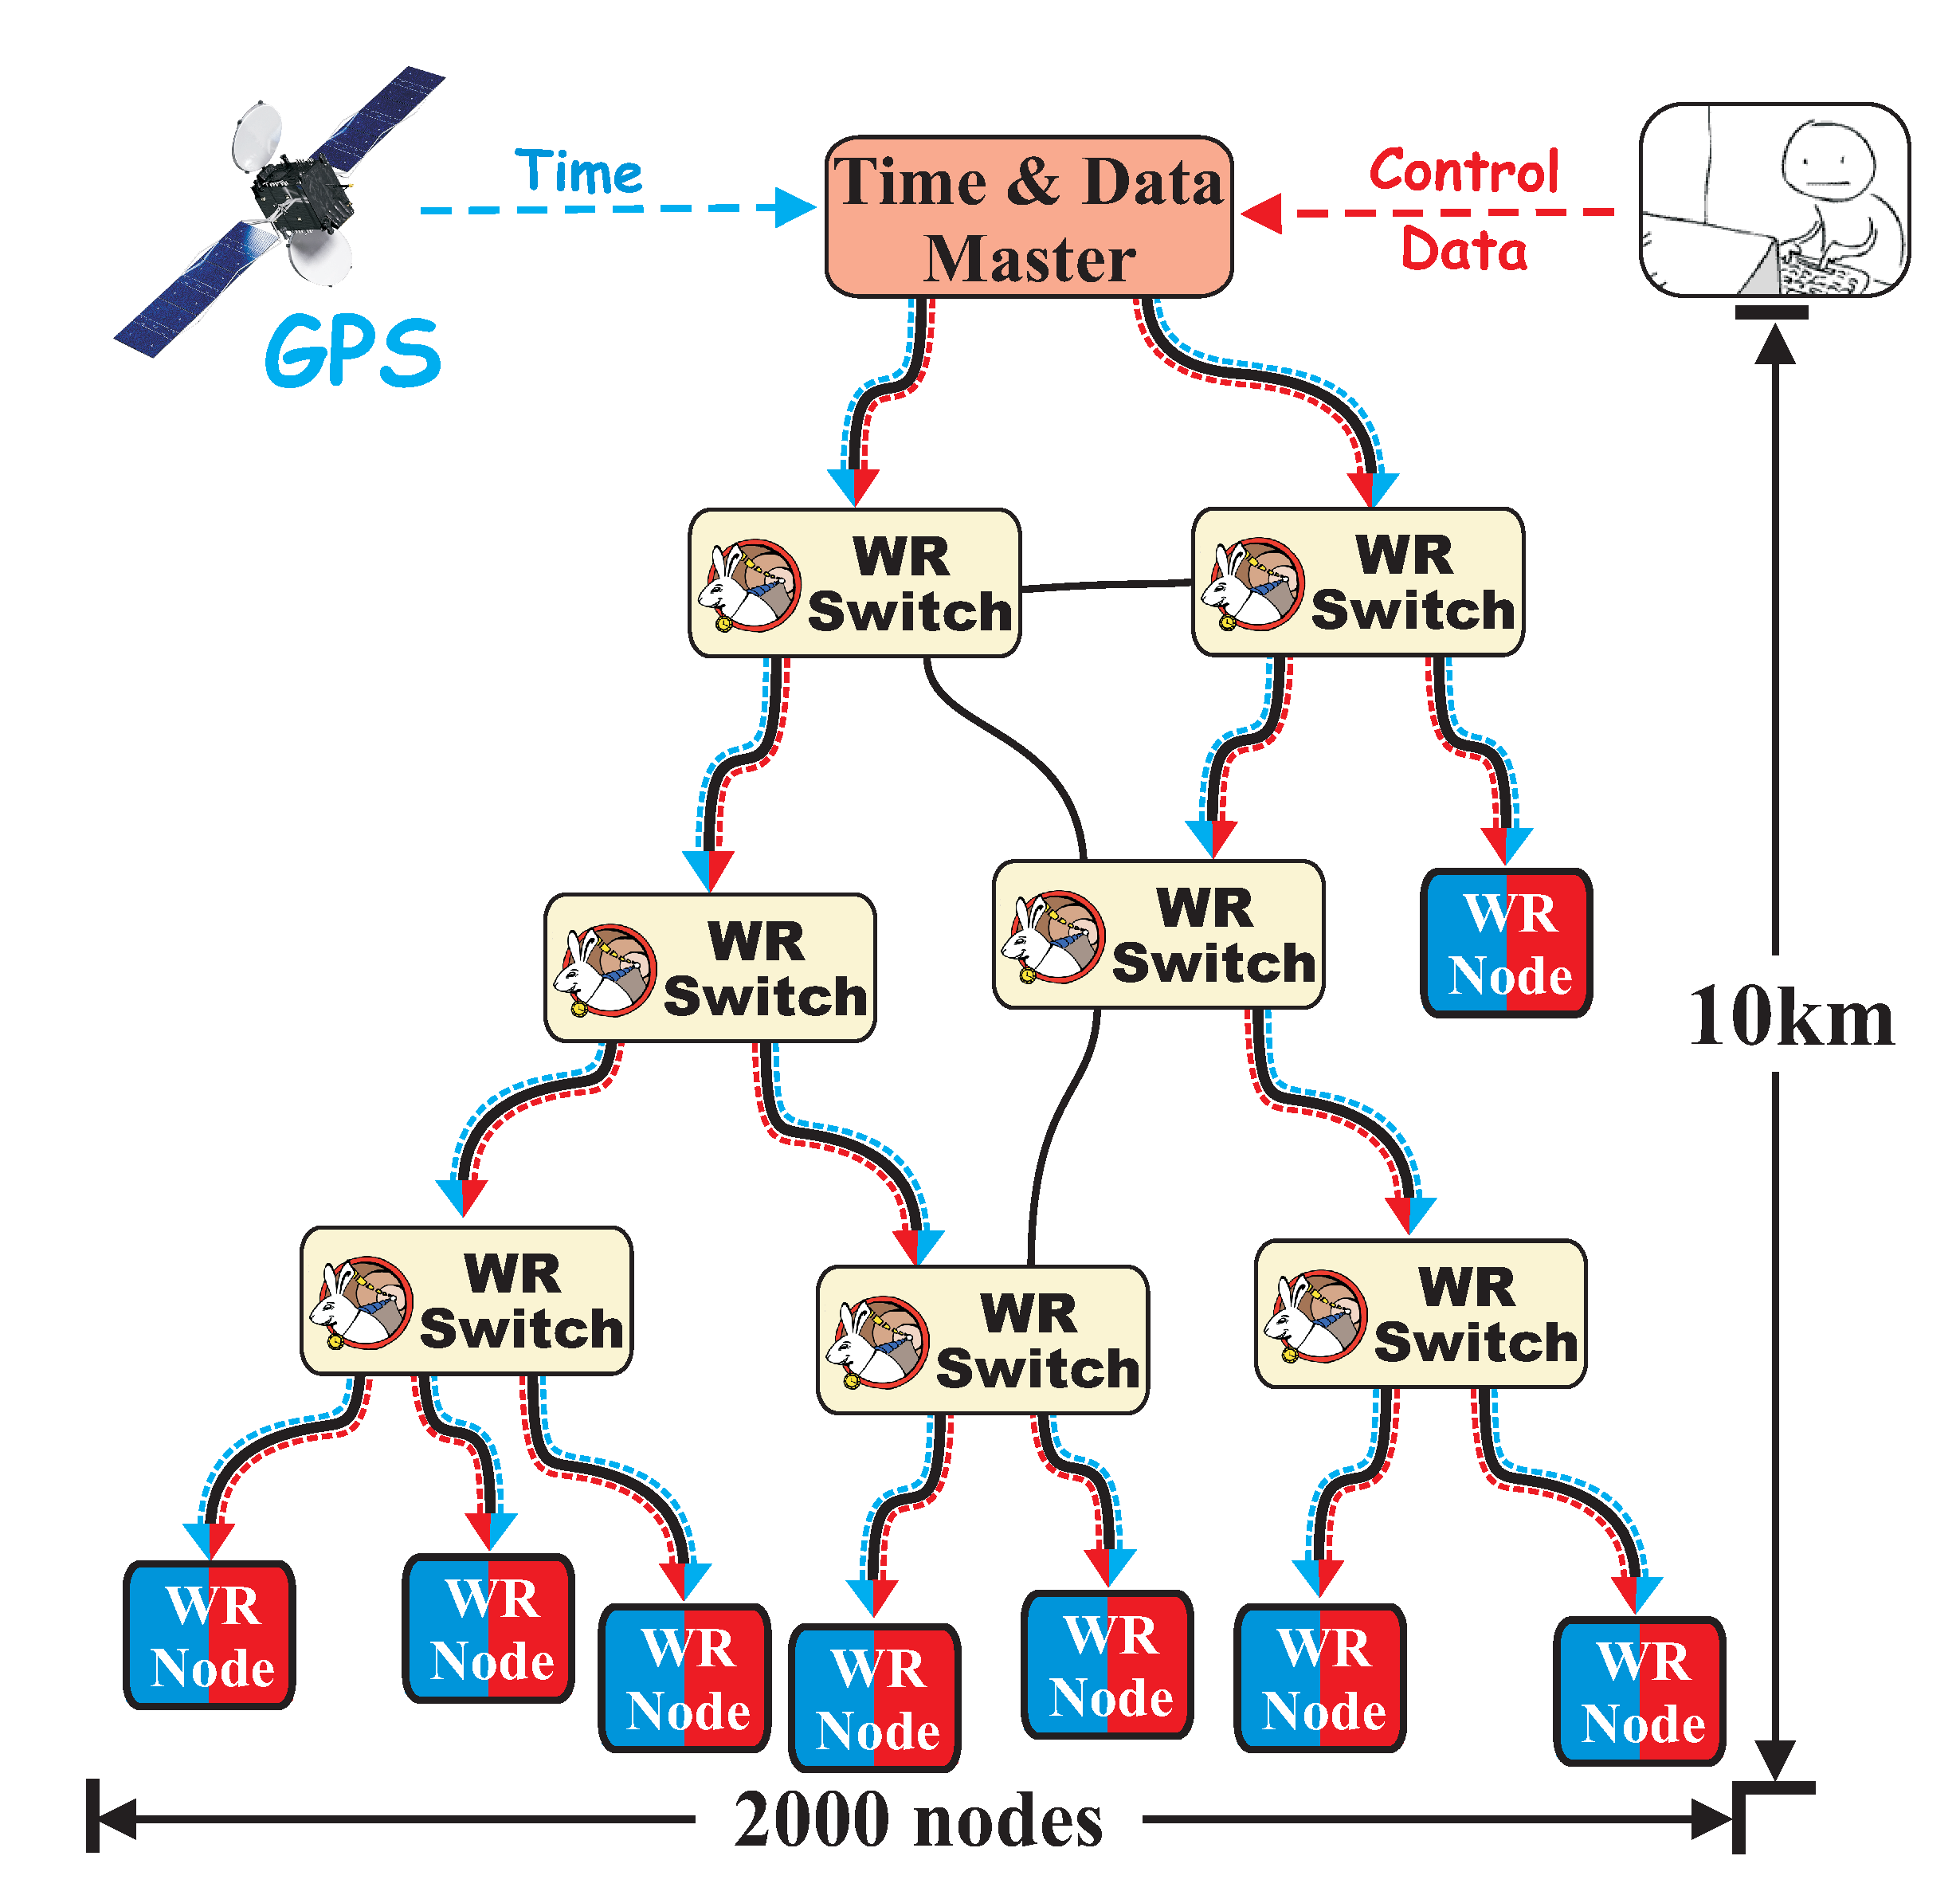
\includegraphics[height=1.0\textwidth]{network/wr_network-new.pdf}
    \end{center}
\end{columns}
  

\end{frame}
%%%%%%%%%%%%%%%%%%%%%%%%%%%%%%%%%%%%%%%%%%%%%%%%%%%%%%%%%%%%%%%%%%%%%%%%%%%%%%%%%%%%%%%%%%%%%%%%%%%%
\section{Reliability in a White Rabbit Network}
% \subsection{}
%%%%%%%%%%%%%%%%%%%%%%%%%%%%%%%%%%%%%%%%%%%%%%%%%%%%%%%%%%%%%%%%%%%%%%%%%%%%%%%%%%%%%%%%%%%%%%%%%%%%
\begin{frame}{Reliability in a White Rabbit Network}


    \begin{center}
    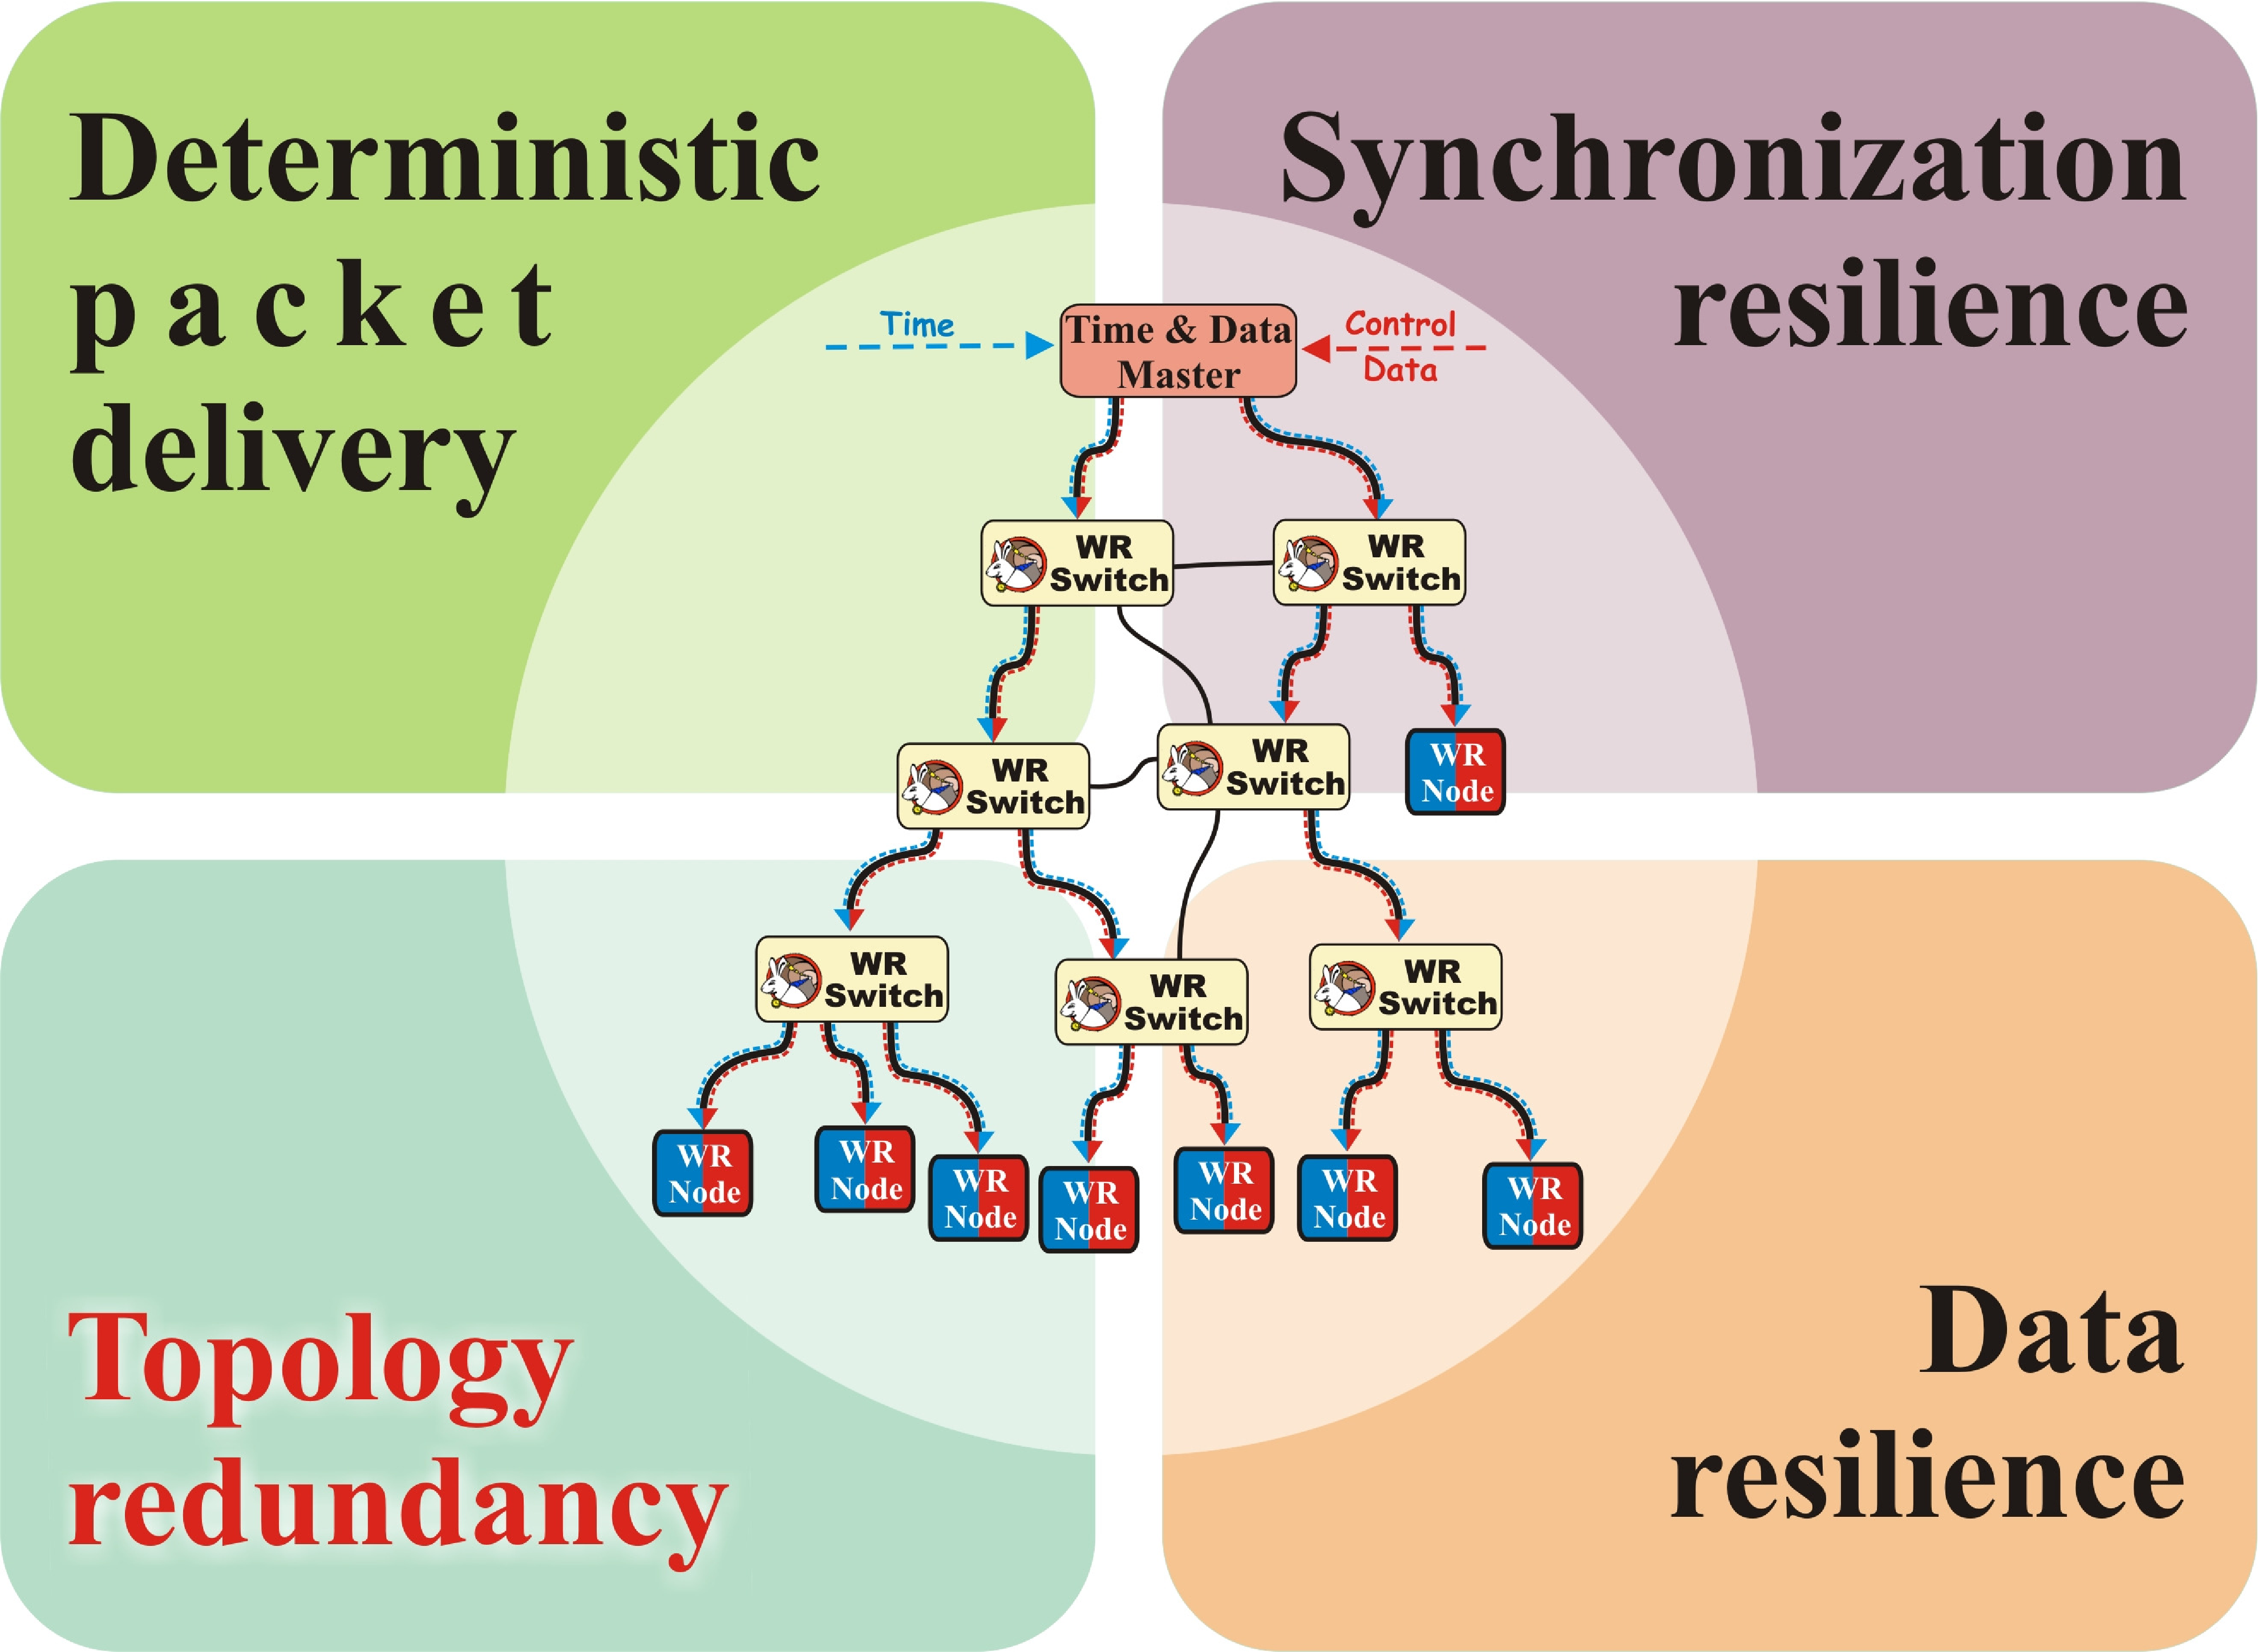
\includegraphics[width=0.9\textwidth]{robustness/sub_domains-old.pdf}
    \end{center}

  

\end{frame}



\end{document}
